\documentclass{article}

\usepackage{fancyhdr}
\usepackage{extramarks}
\usepackage{amsmath}
\usepackage{amsthm}
\usepackage{amsfonts}
\usepackage{tikz}
\usepackage[plain]{algorithm}
\usepackage{algpseudocode}
\usepackage{longtable} %for longtabu
\usepackage{tabu} %for longtabu
\usepackage{hhline} %for double \hline in longtabu
\usepackage{hyperref}
\usepackage{changepage}
\bibliography{refs}
\bibliographystyle{ieee}

\usetikzlibrary{automata,positioning}

%
% Basic Document Settings
%

\topmargin=-0.45in
\evensidemargin=0in
\oddsidemargin=0in
\textwidth=6.5in
\textheight=9.0in
\headsep=0.25in

\linespread{1.1}

\pagestyle{fancy}
\lhead{\hmwkAuthorName}
\rhead{COMS 412 Final Project Report }
\lfoot{\lastxmark}
\cfoot{\thepage}

\renewcommand\headrulewidth{0.4pt}
\renewcommand\footrulewidth{0.4pt}

\setlength\parindent{0pt}

%
% Create Problem Sections
%

\setcounter{secnumdepth}{0}
\newcounter{partCounter}
\newcounter{homeworkProblemCounter}
\setcounter{homeworkProblemCounter}{1}
\nobreak\extramarks{Problem \arabic{homeworkProblemCounter}}{}\nobreak{}

%
% Homework Problem Environment
%
% This environment takes an optional argument. When given, it will adjust the
% problem counter. This is useful for when the problems given for your
% assignment aren't sequential. See the last 3 problems of this template for an
% example.
%

%
% Homework Details
%   - Title
%   - Due date
%   - Class
%   - Section/Time
%   - Instructor
%   - Author
%

\newcommand{\hmwkTitle}{Final Project}
\newcommand{\hmwkClass}{COMS 412}
\newcommand{\hmwkClassInstructor}{Various Concurrency Experiments with Probabilistic Model Checking}
\newcommand{\hmwkAuthorName}{\textbf{Charles Dudley}}

%
% Title Page
%

\title{
    \vspace{2in}
    \textmd{\textbf{\hmwkClass:\ \hmwkTitle}}\\
    \vspace{0.1in}\large{\textbf{\hmwkClassInstructor \hmwkClassTime}}
    \vspace{3in}
}

\author{\hmwkAuthorName}
\date{}

\renewcommand{\part}[1]{\textbf{\large Part \Alph{partCounter}}\stepcounter{partCounter}\\}

%
% Various Helper Commands
%

% Useful for algorithms
\newcommand{\alg}[1]{\textsc{\bfseries \footnotesize #1}}

% For derivatives
\newcommand{\deriv}[1]{\frac{\mathrm{d}}{\mathrm{d}x} (#1)}

% For partial derivatives
\newcommand{\pderiv}[2]{\frac{\partial}{\partial #1} (#2)}

% Integral dx
\newcommand{\dx}{\mathrm{d}x}

% Alias for the Solution section header
\newcommand{\solution}{\textbf{\large Solution}}

% Probability commands: Expectation, Variance, Covariance, Bias
\newcommand{\E}{\mathrm{E}}
\newcommand{\Var}{\mathrm{Var}}
\newcommand{\Cov}{\mathrm{Cov}}
\newcommand{\Bias}{\mathrm{Bias}}

\def\until{\hspace*{0.1cm} \mathcal{U} \hspace*{0.1cm}}

\def\next {\hspace*{0.1cm} \mathcal{X}}

\def\release{\hspace*{0.1cm} \mathcal{R} \hspace*{0.1cm}}

\def\allpaths{\mathcal{A}}
\def\existspath{\mathcal{E}}

\begin{document}
\maketitle
\pagebreak
\section{Introduction}

For safety critical systems, testing is simply an insufficient method of assessing correctness. Testing is a very limited method of analysis in that it can only find the bugs you look for. A robust test suite can be generated for a system which still misses some critical error in implementation. For \textit{safety critical systems} (systems where failure is extremely costly), we cannot afford  for errors to slip past our testing. Examples might include an air traffic control system, where any fault could cost hundreds lives, or the software controlling a satellite launched away into space, which could cost untold millions of dollars if it were to crash.  \\

Formal Verification is a powerful tool used in verifying the correctness and reliability of safety critical systems which can account for the shortcomings of traditional testing. Formal Verification techniques such as \textit{Model Checking} are a more robust method of analysis that involves the exploration of a system's entire state space. These techniques can be used to discover errors in implementation and/or specification which may easily be missed by any test generation technique. When applied effectively, model checking can provide absolute proofs of an implementation's alignment to given specifications (these determinations are referred to as \textit{correctness}). A model checker's proof of correctness can be a very powerful safety guarantee for smaller systems, but for many systems it is very difficult (or not practical) to achieve such a guarantee. Firstly, for many systems it is simply impossible to explore the entire state space with a reasonable amount of compute and memory. 
Models of systems can easily contain trillions of states, in which case verification of a property over the entire system is very difficult. These systems still may be analyzed by applying simplifications to the model of the system, but the guarantees resulting from verification on the simplified model may not transfer to the real system.
Additionally, many systems involve a level of uncertainty that clouds the definitive \textit{yes/no} property satisfaction we would like to assert on systems. The behavior of a system is likely influenced by the environment it operates in. For instance, the performance of a self-driving car is affected by the accuracy of its computer vision processing (a probabilistic process itself), the conditions of the road surface, and behavior of other (potentially manually operated) vehicles. These external influences on the behavior of a system are very difficult to capture in traditional verification methods, but may be extremely valuable in assessing the safety of that system. These systems may still be analyzed by applying certain assumptions to the environment, such as modeling the road surface conditions as a markovian process.\\

In this report I present a study of multiple applications of probabilistic model checking to real world scenarios, such as air traffic control systems. I use PRISM model checker and PRISM specification language to model and analyze these systems. For each system I provide quantitative analysis of safety properties.\\

Included is a \href{https://github.com/chuckdud/COMS412-Final-Project}{GithHub repository} containing all source code for this project. The repository includes a \texttt{.devcontainer} directory which can be used to start an editing environment inside a Docker container including all of the project dependencies. Instructions on how to start this environment can be found \href{https://code.visualstudio.com/docs/devcontainers/containers}{here}.

\section{Terminology}
1. \textbf{Discrete-Time Markov Chain}: \\

A \textit{Discrete-Time Markov Chain} (DTMC) is a stochastic process which models the behavior of some process external to our \textit{agent}. DTMCs are represented as finite state machines where every transition is assigned a probability value between 0 and 1. For a DTMC, a transition from one state to another is controlled entirely by the transition probabilities of the system. Behavior of this model can be predicted and analyzed without any modification. \\

DTMC $M_c$ is formally defined as $M_c: (S, \sigma, s_0, \Sigma, L)$ with 
\begin{itemize}
    \setlength\itemsep{0em}
    \item Probability transition function, $\sigma: S \times S \rightarrow [0, 1]$
    \item Initial state, $s_0$
    \item Set of atomic propositions, $\Sigma$
    \item Labeling function, $L$
\end{itemize}

2. 1. \textbf{Agent}: A decision-making entity in a scenario. The agent is capable of making non-deterministic decisions, called \textit{actions}.\\

3. \textbf{Markov Decision Process}:

A \textit{Markov Decision Process} (MDP) is a stochastic process modeling the behavior of a \textit{non-deterministic agent}. MDPs are represented as finite state machines with each transition assigned an \textit{action} as well as a probability value between 0 and 1. 

An agent (modeled with an MDP) must \textit{non-deterministically} select an \textit{action} with every state transition. This action may affect the probability transition function, therefore behavior cannot be predicted in isolation.

Markov Decision Process $M_p$ is formally defined as $M_p: (S, s_0, A, \sigma, \Sigma, L)$ with
\begin{itemize}
    \setlength\itemsep{0em}
    \item Set of states, $S$
    \item Initial state, $s_0 \in S$
    \item Finite set of actions, $A$
    \item Probability transition function, $\sigma: S \times A \times S \rightarrow [0, 1]$
    \item Set of atomic propositions, $\Sigma$
    \item Labeling function, $L$
\end{itemize}
4. \textbf{Policy}: A rule, which when applied to an MDP, resolves the non-determinism in the system. A policy is essentially a list of rules which the agent must follow, specifying an action the agent must take under certain conditions. Application of a policy to an MDP reduces it to a deterministic system which we can reason about more effectively. \\

5. \textbf{Parallel Composition}: A system which models the joint behavior of multiple (synchronized) independent systems. \\

A parallel composition of an MDP, $M_p: (S_p, s_{0p}, A, \sigma_p, \Sigma_p, L_p)$ and an DTMC, $M_c: (S_c, \sigma_c, s_{0c}, \Sigma_c, L_c)$, is defined as 
$M_{||}: (S, s_{00}, A, \sigma, \Sigma, L)$ with
\begin{itemize}
    \setlength\itemsep{0em}
    \item Set of states, $S=S_p \times S_c$
        \begin{itemize}
            \item State $(s_{p},s_{c})\in S$ may be abbreviated to $s_{pc}$
        \end{itemize}
    \item Initial state, $s_{00} = (s_{0p},s_{0c}) \in S$
    \item Finite set of actions, $A$
    \item Probability transition function, $\sigma: S \times A \times S \rightarrow [0, 1]$
        \begin{itemize}
            \item[$\circ$] $\sigma(s_{ix}, a, s_{jy})=\sigma_p(s_i, a, s_j) \times \sigma_c(s_x, s_y)$
        \end{itemize}
    \item Set of atomic propositions, $\Sigma = \Sigma_p\cup\Sigma_c$
    \item Labeling function, $L : S\rightarrow \Sigma$
\end{itemize}

\newpage

A parallel composition of an MDP, $M_x: (S_x, s_x, A_x, \sigma_x, \Sigma_x, L_x)$ and another MDP, $M_y: (S_y, s_y, A_y, \sigma_y, \Sigma_y, L_y)$, is defined as 
$M_{||}: (S, s_{xy}, A, \sigma, \Sigma, L)$ with
\begin{itemize}
    \setlength\itemsep{0em}
    \item Set of states, $S=S_x \times S_y$
        \begin{itemize}
            \item State $(s_x,s_y)\in S$ may be abbreviated to $s_{pc}$
        \end{itemize}
    \item Initial state, $s_{xy} = (s_x,s_y) \in S$
    \item Finite set of actions, $A=A_x\cup A_y$
    \item Probability transition function, $\sigma: S \times A_x \times A_y \times S \rightarrow [0, 1]$
        \begin{itemize}
            \item[$\circ$] $\sigma(s_{im}, a_x, a_y, s_{jn})=\sigma_x(s_i, a_x, s_j) \times \sigma_y(s_m, a_y, s_n)$
        \end{itemize}
    \item Set of atomic propositions, $\Sigma = \Sigma_p\cup\Sigma_c$
    \item Labeling function, $L : S\rightarrow \Sigma$
\end{itemize}

\section{Tools}
\subsection{PRISM}

PRISM is both a \textit{specification language} and a \textit{probabilistic model checker}. Both forms of PRISM are used in this project to conduct probabilistic analysis on a series of probabilistic systems. \\

PRISM (specification language) provides simple and concise syntax for defining deterministic and non-deterministic systems, such as DTMCs and MDPs. A system can be defined by its state variables, actions (if necessary), probability transition function. This is how all models are defined for this project. Statements defining the probability transition function will include \textit{action labels}, \textit{guard clauses}, and \textit{transition bodies}. The \textit{action label} is a string which restricts a transition to be made only when a particular action is selected. The \textit{guard clause} is a boolean expression which defines the conditions under which a transition is enabled. The \textit{transition body} of this statement defines the probabilities for making certain transitions; An entire transition definition might look like:

\begin{verbatim}
    [go] a != 5 & a != 8 -> 
                .85: (a'=a+1) + 
                .15: (a'=a)   ;
\end{verbatim}

PRISM enables automatic parallel composition of multiple independent systems, regardless of their deterministic/non-deterministic nature. This is a very powerful feature for models which include interaction between several entities and is a large reason why PRISM was selected as the modeling language. \\

PRISM also enables analysis of systems using PCTL/PLTL specifications. Specifications used in this research take the form of $P_{max}=?[\phi]$, for some LTL expression $\phi$. This specification can be used to compute the maximum probability that a system may satisfy a specification; In this computation, PRISM (model checker) can generate an optimal policy for a non-deterministic system. This optimal policy allows for reasoning about the maximum (or minimum) safety guarantee of a system with respect to $\phi$. \\

For a PRISM model implemented in \texttt{example.pm} and a specification file implemented in \texttt{example.specs}, PRISM model checking can be performed over this system using the following command:
\begin{verbatim}
    $ prism example.pm example.specs
\end{verbatim}

Optionally, PRISM can be configured to output an optimal policy with command line option \texttt{--exportstrat stdout}, though this forces PRISM to use \textit{explicit-state model checking}, which drastically increases the memory required to perform verification.

\newpage
\section{Overview of Scenarios}
\subsection*{Scenario 1: Around the Storm}

For this scenario we will consider a single non-deterministic agent and its interaction with a probabilistic environment. \\

\textbf{Visualization:}

\begin{center}
    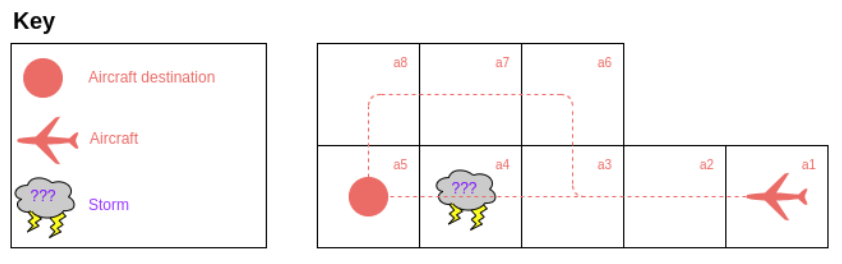
\includegraphics[scale=.4]{figs/around_the_storm.png}
    % TODO:: add figure label!!
\end{center}

\textbf{Description:}

An \textit{aircraft} is travelling along a planned trajectory at a constant rate. The planned trajectory, $T$, follows along locations $[a_1,a_2,a_3,a_4,a_5]$ (without making any maneuvers), which is the optimal path from initial location, $a_1$, to destination, $a_5$. \\

There is a certain probability that a \textit{storm} will occur along the planned trajectory (in location $a_3$), making the planned trajectory dangerous for air travel. In this case, the aircraft should maneuver to follow a safe trajectory, $T'$. This alternate trajectory traverses along locations $[a_1,a_2,a_3,a_6,a_7,a_8,a_5]$. The aircraft may fail to execute this maneuver.\\

In order to minimize cost, trajectory $T$ is preferred. However, a maneuver should be executed by the aircraft if it is on course for dangerous airspace (the storm). \\

\textit{Aside}: Although very simple, this model can provide interesting insights into expected behavior of a probabilistic system. Results and practices from this example may be expanded upon to model much more interesting scenarios, as will be explored in later sections. \\


\textbf{Specifications:}

In order to conduct analysis over this system, specifications of desired/undesired behavior must be drafted. A few examples of English specifications:
\begin{itemize}
    \setlength\itemsep{0em}
    \item The aircraft always eventually reaches its destination.

    \item The aircraft reaches its destination without entering the storm.

    \item The aircraft reaches its destination without entering the storm while only changing course to avoid a storm.

    \item The aircraft enters the storm.
\end{itemize}

For probabilistic analysis, these specifications must be revised to the following form:

\begin{itemize}
    \setlength\itemsep{0em}
    \item What is the maximum probability the aircraft always eventually reaches its destination?

    \item What is the maximum probability the aircraft can reach its destination without entering the storm?

    \item What is the maximum probability the aircraft can reach its destination without entering the storm, given it never changes course except to avoid a storm?

    \item What is the maximum probability the aircraft enters the storm?
\end{itemize}

\subsection*{Scenario 2: Air Traffic Control}

For this scenario we will consider the interaction between two non-deterministic agents. \\

\textbf{Visualization:}

\begin{center}
    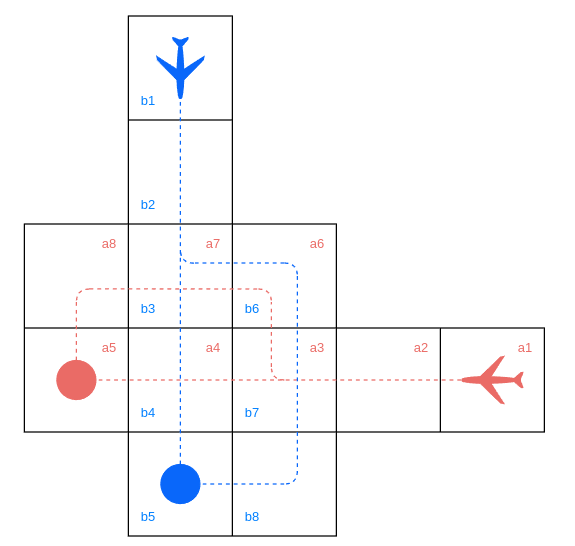
\includegraphics[scale=.4]{figs/air_traffic_control.png}
\end{center}

\textbf{Description:}

An aircraft, \textit{pink}, is travelling along a planned trajectory at a constant rate. The planned trajectory, $T_{p}$, follows along locations $[a_1, a_2, a_3, a_4, a_5]$ (without making any maneuvers), which is the optimal path from initial location, $a_1$, to destination, $a_5$.\\

Another similar aircraft, \textit{blue}, is also travelling along its planned trajectory at the same rate. This planned trajectory, $T_{b}$, follows along locations $[b_1, b_2, b_3, b_4, b_5]$ (without making any maneuvers), which is the optimal path from initial location, $b_1$, to destination, $b_5$. \\

Trajectories $T_p$ and $T_b$ intersect in $a_4/b_4$, creating a potential collision. This collision is highly likely due to the aircraft's initial speeds and distances from $a_4/b_4$. In order to avoid a potential collision, either aircraft may maneuver into their alternate trajectory. For \textit{pink} this alternate trajectory, $T_p'$, is $[a_1, a_2, a_3, a_6, a_7, a_8, a_5]$. For \textit{blue} this alternate trajectory, $T_b'$, is $[b_1, b_2, b_3, b_6, b_7, b_8, b_5]$. Either aircraft may fail to execute their maneuver. \\

Similarly to the Storm Avoidance scenario, each aircraft should prefer their initial trajectory in navigating to their destination to minimize cost. However, a maneuver must be executed if a collision is imminent. \\

\textbf{Specifications:}

Some interesting specifications for analysis of this system:
\begin{itemize}
 \item Each aircraft reaches its respective destination.

 \item Each aircraft reaches its respective destination without a collision.

 \item Each aircraft reaches its respective destination without a collision, executing a maneuver only to avoid an imminent collision.

 \item A collision eventually occurs in some specific cell $a_xb_y$.

 \item A collision occurs in any cell.
\end{itemize}

Similarly to the \textbf{Around the Storm} scenario, these specifications must be rewritten into an inquisitive form (\textit{What is the maximum probability of $X$?}) to allow for probabilistic analysis of these properties.

\subsection*{Scenario 3: Through The Storm}

For this scenario we will, again, consider the interaction between a single non-deterministic agent and its deterministic environment. \\

\textbf{Visualization:}

\begin{center}
    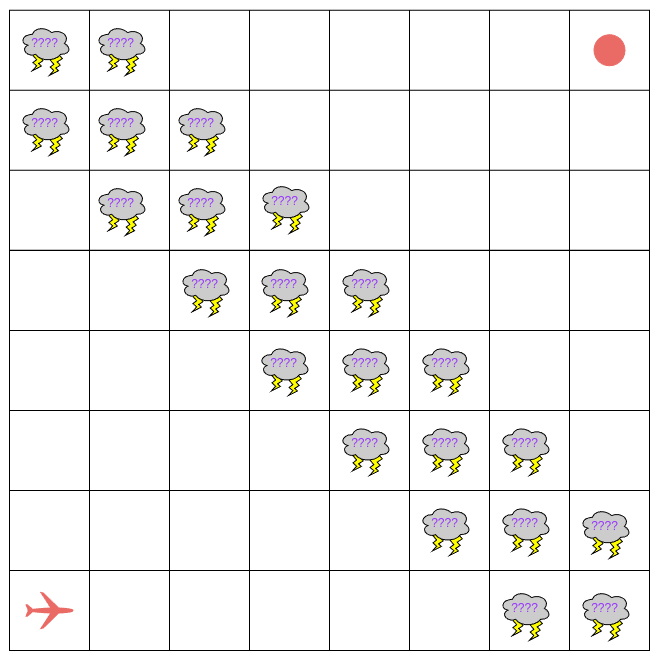
\includegraphics[scale=.4]{figs/through_the_storm.png}
\end{center}

\textbf{Description:}

An \textit{aircraft} is initially travelling East from position (0,0). In order to reach its destination, the aircraft must navigate from its initial position to its destination, (8,8). This aircraft is capable of turning to travel Northward or Eastward, or continuing in its current direction, but it is forbidden from turning in any other direction. \\

In order to reach its destination, the aircraft must pass through a \textit{storm} which spans the entire airspace. Due to the severity of the storm, the aircraft may only sustain itself for a limited period of time inside of the storm. Therefore it is critical that the aircraft navigate through the dangerous airspace while minimizing its time spent inside the storm.
\\

\textbf{Specifications:}

Some interesting probabilistic specifications for analysis of this system:
\begin{itemize}
 \item The aircraft eventually reaches its destination.

 \item The aircraft eventually reaches its destination without entering a storm.

 \item The aircraft eventually reaches its destination while minimizing contact with storms below some threshold, $\psi$.
\end{itemize}

Similarly to previous scenarios, these specifications must be rewritten into an inquisitive form (\textit{What is the maximum probability of $X$?}) to allow for probabilistic analysis of these properties.


\section{Modeling the Scenarios}
\subsection*{Scenario 1: Around The Storm}

The behavior of the \textbf{\textit{storm}} will be modeled by a DTMC, $M_c$ as follows:

\begin{center}
    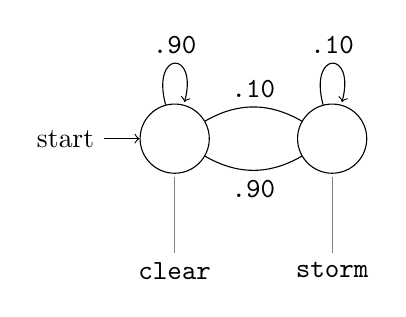
\begin{tikzpicture}
        \node [state, pin={[pin distance=1cm, pin edge={-, shorten <= 1pt}]below:\texttt{clear}}, initial] (s0) at (0,0) {};
        \node [state, pin={[pin distance=1cm, pin edge={-, shorten <= 1pt}]below:\texttt{storm}}] (s1) at (2,0) {};
    \draw
        (s0) edge[above, bend left] node[] {\texttt{.10}} (s1)
        (s1) edge[below, bend left] node[] {\texttt{.90}} (s0)
        
        (s0) edge[loop above] node[] {\texttt{.90}} (s0)
        (s1) edge[loop above] node[] {\texttt{.10}} (s1);
    \end{tikzpicture}
\end{center}

This DTMC has two states, corresponding to the status of the airspace in $a_4$: \textit{clear} or \textit{stormy} skies. The skies are initially \textit{clear} and tend to change state with low probability (0.10). \\

\textit{Aside}: This is clearly a gross oversimplification of the behavior of a real storm, however simplifications of this magnitude must be applied in order to create a reasonably sized model a system (in fact, even an entity as simple as this one can create state space explosion, as will be detailed in a later section). Simplifications of this sort will be applied to entities in all scenarios, including both \textit{storms} and \textit{aircraft}. \\

The behavior of the \textbf{\textit{aircraft}} will be modeled by an MDP, $M_p$ as follows:
\begin{center}
    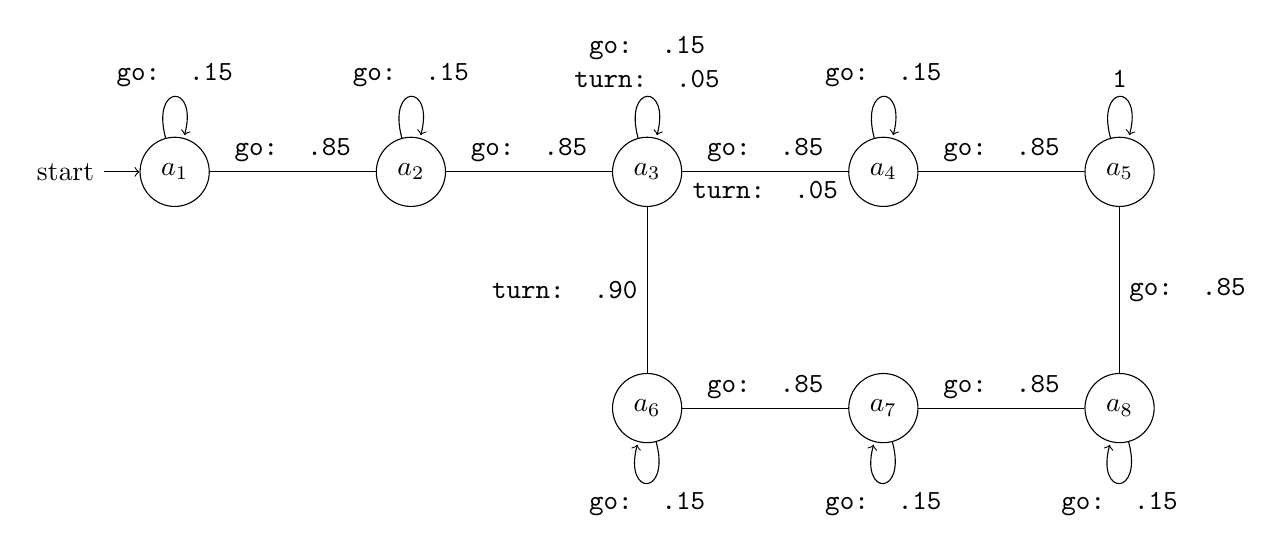
\begin{tikzpicture}
        \node [state, initial] (a1) at (0,0) {$a_1$};
        \node [state] (a2) at (3,0) {$a_2$};
        \node [state] (a3) at (6,0) {$a_3$};
        \node [state] (a4) at (9,0) {$a_4$};
        \node [state] (a5) at (12,0) {$a_5$};
        \node [state] (a6) at (6,-3) {$a_6$};
        \node [state] (a7) at (9,-3) {$a_7$};
        \node [state] (a8) at (12,-3) {$a_8$};
        
    \draw        
        (a1) edge[loop above] node[] {\texttt{go: .15}} (a1)
        (a1) edge[above] node[] {\texttt{go: .85}} (a2)

        (a2) edge[loop above] node[] {\texttt{go: .15}} (a2)
        (a2) edge[above] node[] {\texttt{go: .85}} (a3)
        
        (a3) edge[loop above] node[align=center] {\texttt{go: .15}\\\texttt{turn: .05}} (a3)
        (a3) edge[above] node[align=center] {\texttt{go: .85}} (a4)
        (a3) edge[below] node[align=center] {\texttt{turn: .05}} (a4)
        (a3) edge[left]  node[align=center] {\texttt{turn: .90}} (a6)

        (a4) edge[loop above] node[] {\texttt{go: .15}} (a4)
        (a4) edge[above] node[] {\texttt{go: .85}} (a5)

        (a5) edge[loop above] node[] {\texttt{1}} (a5)

        (a6) edge[loop below] node[] {\texttt{go: .15}} (a6)
        (a6) edge[above] node[] {\texttt{go: .85}} (a7)

        (a7) edge[loop below] node[] {\texttt{go: .15}} (a7)
        (a7) edge[above] node[] {\texttt{go: .85}} (a8)

        (a8) edge[loop below] node[] {\texttt{go: .15}} (a8)
        (a8) edge[right] node[] {\texttt{go: .85}} (a5)
        ;
    \end{tikzpicture}
\end{center}

This MDP has 8 states, representing each of the $a_i$ locations the aircraft may travel through. \\

The two \textit{non-deterministic actions} available to this agent are \texttt{go} and \texttt{turn}. \texttt{go} is an action whose execution results in high probability (0.85) that the aircraft will move directly from its current state $a_i$, to the next state $a_{i+1}$, and a low probability (0.15) that the aircraft will remain in $a_i$. \texttt{go} is enabled in all states except the destination, $a_5$. \texttt{turn} is an action whose execution results in high probability (0.90) of the aircraft altering its trajectory, and a low probability of either remaining in its current position or moving ahead (0.50 for either case). This action is defined only in $a_3$. Execution of a specific action still leads to a probabilistic state transition (i.e.  when executing \texttt{turn}, the aircraft may fail to alter its trajectory).\\

The \textbf{\textit{joint behavior}} of the two independent systems, $M_c$ and $M_p$, can be modeled using a \textit{parallel composition} of the two systems. This parallel composition will be defined as an MDP, $M$, constructed according to the definition given above in \textbf{Terminology}. \\

For the sake of brevity, a depiction of this parallel composition is not provided. \\

A PRISM implementation of this model is included in \texttt{around\_the\_storm/around\_the\_storm.pm}. In this model, the \textit{aircraft} uses state variable $a\in[1..8]$ to store its location, and the storm uses state variable $p\in[0..1]$ to encode its presence/absence. \\

% This resulting system, $M$, will have 16 states (8 states in $M_p$ $\times$ 2 states in $M_c$). Every transition between these states will be labeled with an action from $M_p$, and the probability for each transition $(a_is_m)\rightarrow(a_js_n)$ will be equal to the product of the probabilities of transitions

\subsection{Scenario 2: Air Traffic Control}
The behavior of \textbf{\textit{pink}} will be modeled by an MDP as follows:

\begin{center}
    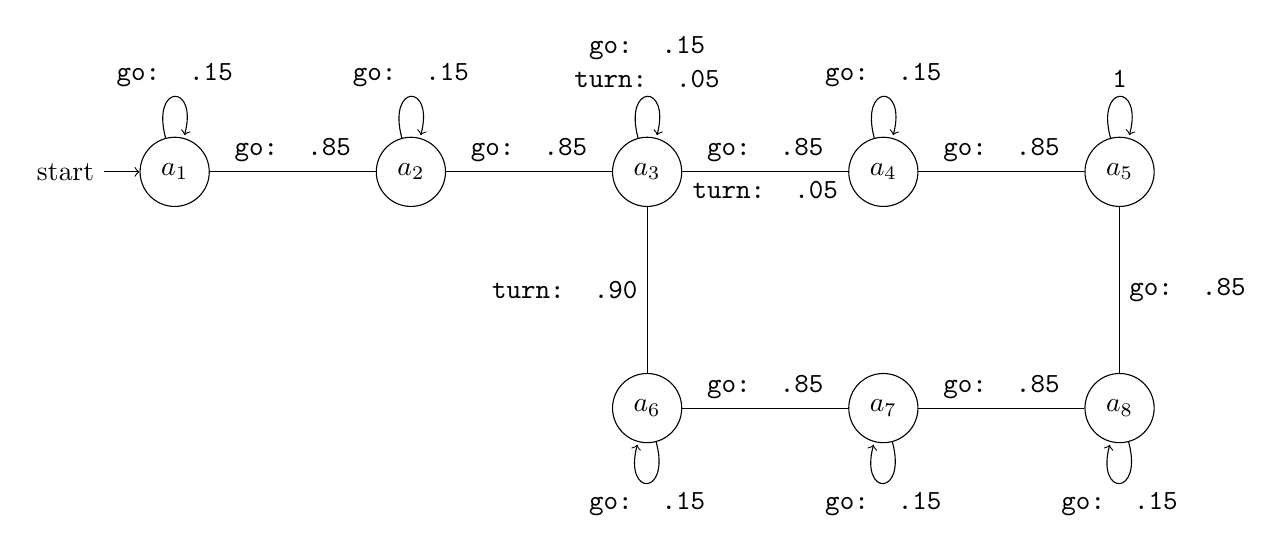
\begin{tikzpicture}
        \node [state, initial] (a1) at (0,0) {$a_1$};
        \node [state] (a2) at (3,0) {$a_2$};
        \node [state] (a3) at (6,0) {$a_3$};
        \node [state] (a4) at (9,0) {$a_4$};
        \node [state] (a5) at (12,0) {$a_5$};
        \node [state] (a6) at (6,-3) {$a_6$};
        \node [state] (a7) at (9,-3) {$a_7$};
        \node [state] (a8) at (12,-3) {$a_8$};
        
    \draw        
        (a1) edge[loop above] node[] {\texttt{go: .15}} (a1)
        (a1) edge[above] node[] {\texttt{go: .85}} (a2)

        (a2) edge[loop above] node[] {\texttt{go: .15}} (a2)
        (a2) edge[above] node[] {\texttt{go: .85}} (a3)
        
        (a3) edge[loop above] node[align=center] {\texttt{go: .15}\\\texttt{turn: .05}} (a3)
        (a3) edge[above] node[align=center] {\texttt{go: .85}} (a4)
        (a3) edge[below] node[align=center] {\texttt{turn: .05}} (a4)
        (a3) edge[left]  node[align=center] {\texttt{turn: .90}} (a6)

        (a4) edge[loop above] node[] {\texttt{go: .15}} (a4)
        (a4) edge[above] node[] {\texttt{go: .85}} (a5)

        (a5) edge[loop above] node[] {\texttt{1}} (a5)

        (a6) edge[loop below] node[] {\texttt{go: .15}} (a6)
        (a6) edge[above] node[] {\texttt{go: .85}} (a7)

        (a7) edge[loop below] node[] {\texttt{go: .15}} (a7)
        (a7) edge[above] node[] {\texttt{go: .85}} (a8)

        (a8) edge[loop below] node[] {\texttt{go: .15}} (a8)
        (a8) edge[right] node[] {\texttt{go: .85}} (a5)
        ;
    \end{tikzpicture}
\end{center}

The behavior of \textbf{\textit{blue}} will be modeled by an identical MDP as follows:

\begin{center}
    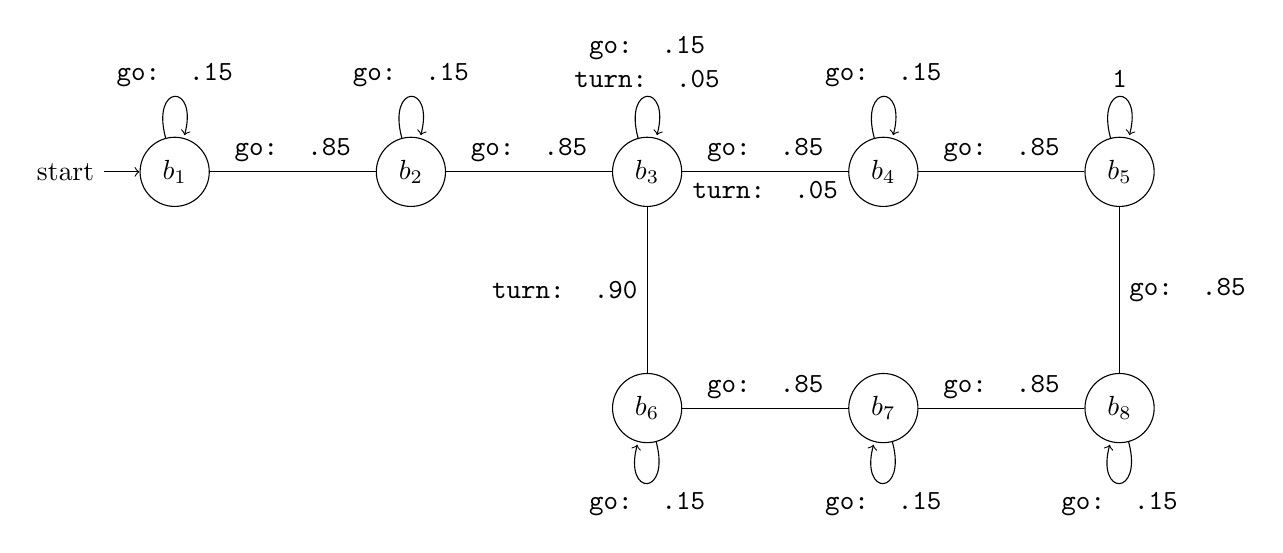
\begin{tikzpicture}
        \node [state, initial] (b1) at (0,0) {$b_1$};
        \node [state] (b2) at (3,0) {$b_2$};
        \node [state] (b3) at (6,0) {$b_3$};
        \node [state] (b4) at (9,0) {$b_4$};
        \node [state] (b5) at (12,0) {$b_5$};
        \node [state] (b6) at (6,-3) {$b_6$};
        \node [state] (b7) at (9,-3) {$b_7$};
        \node [state] (b8) at (12,-3) {$b_8$};
        
    \draw        
        (b1) edge[loop above] node[] {\texttt{go: .15}} (b1)
        (b1) edge[above] node[] {\texttt{go: .85}} (b2)

        (b2) edge[loop above] node[] {\texttt{go: .15}} (b2)
        (b2) edge[above] node[] {\texttt{go: .85}} (b3)
        
        (b3) edge[loop above] node[align=center] {\texttt{go: .15}\\\texttt{turn: .05}} (b3)
        (b3) edge[above] node[align=center] {\texttt{go: .85}} (b4)
        (b3) edge[below] node[align=center] {\texttt{turn: .05}} (b4)
        (b3) edge[left]  node[align=center] {\texttt{turn: .90}} (b6)

        (b4) edge[loop above] node[] {\texttt{go: .15}} (b4)
        (b4) edge[above] node[] {\texttt{go: .85}} (b5)

        (b5) edge[loop above] node[] {\texttt{1}} (b5)

        (b6) edge[loop below] node[] {\texttt{go: .15}} (b6)
        (b6) edge[above] node[] {\texttt{go: .85}} (b7)

        (b7) edge[loop below] node[] {\texttt{go: .15}} (b7)
        (b7) edge[above] node[] {\texttt{go: .85}} (b8)

        (b8) edge[loop below] node[] {\texttt{go: .15}} (b8)
        (b8) edge[right] node[] {\texttt{go: .85}} (b5)
        ;
    \end{tikzpicture}
\end{center}

The \textit{non-deterministic actions} available to \textbf{\textit{pink}} and \textbf{\textit{blue}} are identical to those of the \textbf{\textit{aircraft}} from \textbf{Around The Storm} above. \\

The \textbf{\textit{joint behavior}} of these two independent systems can also be modeled using a \textit{parallel composition}. This resulting system will contain 64 states (8 states in \textit{pink} $\times$ 8 states in \textit{blue}). Additionally, the actions available to this composed system will be pairs of actions selected in each subsystem, ex. \texttt{pink\_go\_blue\_go}, \texttt{pink\_turn\_blue\_go}, etc. (we might think of this composed system as coordinating decision making between the two independent agents). Details of the parallel composition are defined in \textbf{Terminology}. \\

Again, for the sake of brevity the parallel composition is not depicted for this system. A PRISM implementation of this model is included in \texttt{air\_traffic\_control/air\_traffic\_control.pm}. In this model, each aircraft uses a single state variable, $p\in[1..8]$ for \texttt{pink}, $b\in[1..8]$ for \texttt{blue}, to encode its location. The full details of the probability transition function is defined in the source file given above, although each is identical to the aircraft of \textbf{Around the Storm}.
\subsection*{Scenario 3: Through The Storm}
The behavior of the \textbf{\textit{storm}} will be modeled by a parallel composition of many independent \textbf{\textit{storm cells}}. Each cell is  modeled by a DTMC, $M_i$, where each  $M_i$ is defined identically to that of the storm in \textbf{Around The Storm}. The entire \textbf{\textit{storm}} is defined as a parallel composition of its 22 \textit{storm cells}, denoted as $M_0 || M_1 || \cdots || M_{21}$. The resulting state space, $S_{storm}$, has $|S_{storm}|=2^{22}$. \\

The behavior of the \textbf{\textit{aircraft}} will be modeled by an MDP defined as follows: \\

Each state for the aircraft will be defined by its three state variables, $x$, its position relative to the x-axis, $y$, its position relative to the y-axis, and $heading$, the direction the aircraft is facing. Therefore $s\in S_{aircraft}$ takes the form $(x,y,heading)$. For this state space we have $|S_{aircraft}|=128$. \\

The aircraft will be capable of executing actions [\texttt{go}, \texttt{turn\_left}, \texttt{turn\_right}] to navigate through the environment. \texttt{go} allows the aircraft to continue in its current direction. \texttt{turn\_left} allows the aircraft to change from a Eastward trajectory to an Northbound one, and \texttt{turn\_right} allows the opposite trajectory change. The aircraft will only be capable of travelling right (positive $x$) or up (positive $y$) until it reaches the boundary of the environment. Similar to previous examples, execution of a specific action still leads to a probabilistic state transition (i.e.  when executing \texttt{turn\_left}, the aircraft may fail to change its heading). \\

\textbf{Problem}:
The parallel composition required to model the \textit{storm} alone contains $2^{22}$ states; the final parallel composition that models the joint behavior of the \textit{storm} with the \textit{aircraft} contains $2^{29}$ states (that's 536,870,912 states!). This is far too many states for my resources, so a \textbf{state space reduction} is necessary. \\

In order to reduce the state space of this system, the space available to the \textit{aircraft} will be reduced to a 5x5 grid with 9 \textit{storm cells} as follows:

\begin{center}
   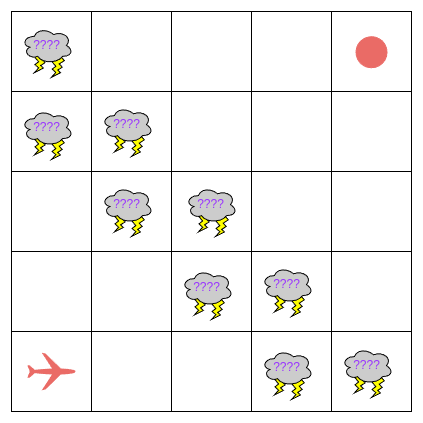
\includegraphics[scale=.4]{figs/restricted.png} 
\end{center}

With unchanged behavior for the \textit{aircraft} and each \textit{storm cell}, the state space of the final parallel composition is reduced to $2^9\times50$ states (down to 25,600). \\

The PRISM implementations for the original system and its restricted version are included in \\\texttt{through\_the\_storm/through\_the\_storm.pm} and \texttt{through\_the\_storm/restricted.pm}, respectively. In each implementation, the aircraft uses two state variables to record its position, $x$ and $y$, and another to record the direction it is facing, \textit{heading}. Each storm requires only one boolean state variable, \textit{present}$_{xy}$ representing whether the storm at $(x,y)$ is present. These PRISM files contain the full details of the probability transition function for this system.

\section{Analyzing The Models}
\subsection*{Scenario 1: Around The Storm}

For \textbf{Around The Storm}, some example specifications were mentioned in \textbf{Overview of Scenarios}. Those can be translated to LTL expressions as follows:
\begin{itemize}
    \item The aircraft always eventually reaches its destination \\
    $\phi_1=\Box\lozenge (a=5)$
    \item The aircraft reaches its destination without entering the storm \\
    $\phi_2=\Box(\lozenge (a=5) \land \lnot(a=4 \land p=1))$
    \item The aircraft reaches its destination without entering the storm while only changing course to avoid a storm \\
    $\phi_3 = \Box(\lozenge (a=5) \land \lnot(a=4 \land p=1) \land (\mathcal{X} (a=6) \implies (p=1)))$
    \item The aircraft enters the storm \\
    $\phi_4 = \lozenge(a=4\land p=1)$
\end{itemize}

Each of the LTL specifications given above can be used to analyze the system in PRISM model checker via the $P_{max}=?$ specification operator. These specifications can be rewritten as $P_{max}=?[\phi_i]$ to compute the policy that maximizes probability of satisfying the specification. These specifications are given in \texttt{around\_the\_storm/around\_the\_storm.specs}.\\

Results from PRISM model checking over the system with these specifications are as follows:
\begin{itemize}
    \item $P_{max}=?[\phi_1]=1.0$
    \item $P_{max}=?[\phi_2]=0.9726029506462466$
    \item $P_{max}=?[\phi_3]=0.8674681337547496$
    \item $P_{max}=?[\phi_4]=0.2819704755353184$
\end{itemize}

PRISM output from these computations is included in \texttt{around\_the\_storm/out.log}.

\subsection*{Scenario 2: Air Traffic Control}

For \textbf{Air Traffic Control}, some English specifications were mentioned in \textbf{Overview of Scenarios}. Those can be translated to LTL expressions as follows:
\begin{itemize}
    \item Each aircraft reaches its respective destination. \\
    $\phi_1= \lozenge (p=5 \land b=5)$
    \item Each aircraft reaches its respective destination without a collision. \\
    $\phi_2= \phi_1 \land \Box\lnot((p=3 \land b=7) \lor (p=4 \land b=4) \lor (p=6 \land b=6) \lor p(=7 \land b=3))$
    \item Each aircraft reaches its respective destination without a collision, executing a maneuver only to avoid an imminent collision. \\
    $\phi_3 = \phi_2 \land (\mathcal{X}(a=6) \implies \mathcal{X}(b=4))$
    \item A collision eventually occurs in some specific cell $a_xb_y$. \\
    $\phi_4 = \lozenge(p=x \land b=y)$
    \item A collision occurs in any cell. \\
    $\phi_5 = \lozenge((p=3 \land b=7) \lor (p=4 \land b=4) \lor (p=6 \land b=6) \lor p(=7 \land b=3))$
\end{itemize}

Similarly to the previous scenario, these LTL expressions can be translated into PRISM probabilistic specification form with use of the $P_{max}=?$ operator. These specifications are given in \\
\texttt{air\_traffic\_control/air\_traffic\_control.specs}.\\

Results from PRISM model checking over the system with these specifications are as follows:
\begin{itemize}
    \item $P_{max}=?[\phi_1] = 1.0$
    \item $P_{max}=?[\phi_2] = 0.9313078531522638$
    \item $P_{max}=?[\phi_3] = 0.9126234014317556$
    \item $P_{max}=?[\phi_4] = 0.0613130758058098$, for $x=7$, $y=3$  
    \item $P_{max}=?[\phi_5] = 0.5761349858270032$
\end{itemize}

PRISM output from these computations is included in \texttt{aair\_traffic\_control/out.log}.

\subsection*{Scenario 3: Through The Storm}

For \textbf{Through the Storm}, English specifications are provided in \textbf{Overview of Scenarios}. Those specifications can be translated to LTL expressions as follows:

\begin{itemize}
 \item The aircraft eventually reaches its destination. \\
 $\phi_1= \lozenge (x=5 \land y=5)$

 \item The aircraft eventually reaches its destination without entering a storm. \\
 $\phi_2= \phi_1 \land \Box\lnot\texttt{damage}$, \\
 for \texttt{damage} defined as $((x = p) \land (y = q) \land $ (\textit{present}$_{pq}$)), $(p,q)\in\{(0,4), (0,3), (1,3), (1,2), (2,2), (2,1), (3,1), (3,0), (4,0)\}$ \\
 (Reminder: \textit{present}$_{pq}$ is the boolean state variable of a storm at $(p,q)$ representing the state of the storm)

 \item The aircraft eventually reaches its destination while minimizing contact with storms below some threshold, $\psi = 2$. \\
 $\phi_3= \phi_1 \land \Box\lnot(\texttt{damage} \land (\mathcal{X}(\lozenge\texttt{damage}))$, \\
  for \texttt{damage} defined as $((x = p) \land (y = q) \land $ (\textit{present}$_{pq}$)), $(p,q)\in\{(0,4), (0,3), (1,3), (1,2), (2,2), (2,1), (3,1), (3,0), (4,0)\}$
 (Reminder: \textit{present}$_{pq}$ is the boolean state variable of a storm at $(p,q)$ representing the state of the storm
\end{itemize}

Similarly to the previous scenarios, these LTL expressions can be translated into PRISM probabilistic specification form with use of the $P_{max}=?$ operator. These specifications are given in \\
\texttt{through\_the\_storm/through\_the\_storm.specs}.\\

Results from PRISM model checking over the system with these specifications are as follows:
\begin{itemize}
    \item $P_{max}=?[\phi_1] = 1.0$
    \item $P_{max}=?[\phi_2] = 0.4692561170484501$
    \item $P_{max}=?[\phi_3] = 0.8267056300097458$
\end{itemize}

PRISM output from these computations is included in \texttt{through\_the\_storm/out.log}.

\section{Results}

For each of the models, \textbf{Around the Storm}, \textbf{Air Traffic Control}, and \textbf{Through the Storm}, I have compiled a series of specifications and their maximum probability of satisfaction in their respective models. Each result gives insight into the properties of each system and allows for reasoning about how effective an agent may behave. Of course, all of these models are "toys" in that they bare little connection to real systems.  However, the practices used in these analyses to measure the probabilistic properties of each of these models serves as a proof of concept which could be applied to real, more complex, systems. \\

Interesting results to note include analysis of $\phi_1$ in each model. $\phi_1$ represented the specification of "agent reaches its destination", and every analysis of this specification resulted in probability $1.0$. This is due to the implementation of the agents as I did not implement proper transitions for "crashes". Also an interesting result is \textbf{Air Traffic Control's} $\phi_5$ which represents the worst case behavior of this system; This case could represent a malicious actor who has taken control of our air traffic control system, and details exactly how likely they are to succeed in their attack.

\section{Extra Experimentation}

To extend my research and learning in probabilistic analysis, I also took on another, somewhat unrelated, problem to solve. There is a dice game which is well liked among my family, called "6-5-4" or "Ship-Captain-Crew" for which I was interested in computing an optimal policy. The rules for this game are defined in detail \href{https://en.wikipedia.org/wiki/Ship,_captain,_and_crew}{here}. \\

I made an effort to model this game as an MDP which I could analyze with respect to specifications such as "What is the maximum probability of ending with the of score 27?" or "What is the maximum probability of ending with a score greater than 20?" (these PRISM specifications are included in \texttt{654/654.specs}). I have included (what I believe to be) a working implementation of this game in \texttt{654/654.pm}, however I have not been able to validate my implementation. Additionally, the policy generated by PRISM is not as useful as I had initially hoped, likely because I poorly chose a game which does not involve many player-actions. \\

Output from PRISM computations over this model for the specifications mentioned just above is contained in \texttt{654/out.log}.

\newpage
\section{Bibliography}

\begin{enumerate}
    \item M. Kwiatkowska and G. Norman and D. Parker, 2011, \textit{PRISM 4.0: Verification of Probabilistic Real-time Systems}
    \item T. Wongpiromsarn and R. D. Murray, 2020, Course Material for EECI\_IGSC-2020
    \item Schäffeler, Maximilian and Abdulaziz, Mohammad, June 2023, \textit{Formally Verified Solution Methods for Markov Decision Processes}
    \item Hansson, Hans and Jonsson, Bengt, 1994, \textit{A logic for reasoning about time 
    and reliability}
    \item Tingting Han and Katoen, J.-P. and Berteun, D., 2009 \textit{Counterexample generation in probabilistic model checking}
    \item Lacerda, Bruno and Parker, David and Hawes, Nick, 2014, \textit{Optimal and dynamic planning for Markov decision processes with co-safe Properties}
\end{enumerate}


\bibliographystyle{ieee}
\nocite{*}
\end{document}
